%-----------------------------------------------------------------------------------------------------------------------------------------------%
%	The MIT License (MIT)
%
%	Copyright (c) 2014 Jan Küster
%
%	Permission is hereby granted, free of charge, to any person obtaining a copy
%	of this software and associated documentation files (the "Software"), to deal
%	in the Software without restriction, including without limitation the rights
%	to use, copy, modify, merge, publish, distribute, sublicense, and/or sell
%	copies of the Software, and to permit persons to whom the Software is
%	furnished to do so, subject to the following conditions:
%	
%	The above copyright notice and this permission notice shall be included in
%	all copies or substantial portions of the Software.
%	
%	THE SOFTWARE IS PROVIDED "AS IS", WITHOUT WARRANTY OF ANY KIND, EXPRESS OR
%	IMPLIED, INCLUDING BUT NOT LIMITED TO THE WARRANTIES OF MERCHANTABILITY,
%	FITNESS FOR A PARTICULAR PURPOSE AND NONINFRINGEMENT. IN NO EVENT SHALL THE
%	AUTHORS OR COPYRIGHT HOLDERS BE LIABLE FOR ANY CLAIM, DAMAGES OR OTHER
%	LIABILITY, WHETHER IN AN ACTION OF CONTRACT, TORT OR OTHERWISE, ARISING FROM,
%	OUT OF OR IN CONNECTION WITH THE SOFTWARE OR THE USE OR OTHER DEALINGS IN
%	THE SOFTWARE.
%	
%
%-----------------------------------------------------------------------------------------------------------------------------------------------%


%============================================================================%
%
%	DOCUMENT DEFINITION
%
%============================================================================%

%we use article class because we want to fully customize the page and dont use a cv template
\documentclass[10pt,A4]{article}	


%----------------------------------------------------------------------------------------
%	ENCODING
%----------------------------------------------------------------------------------------

%we use utf8 since we want to build from any machine
\usepackage[utf8]{inputenc}		

%----------------------------------------------------------------------------------------
%	LOGIC
%----------------------------------------------------------------------------------------

\usepackage{xifthen}% provides \isempty test

%----------------------------------------------------------------------------------------
%	FONT
%----------------------------------------------------------------------------------------

% some tex-live fonts - choose your own
%\usepackage[defaultsans]{droidsans}
%\usepackage[default]{comfortaa}
%\usepackage{cmbright}
\usepackage[default]{raleway}
%\usepackage{fetamont}
%\usepackage[default]{gillius}
%\usepackage[light,math]{iwona}
%\usepackage[thin]{roboto} 

% default the font
\renewcommand*\familydefault{\sfdefault} 	
\usepackage[T1]{fontenc}

%more font size definitions
\usepackage{moresize}		


%----------------------------------------------------------------------------------------
%	PAGE LAYOUT  DEFINITIONS
%----------------------------------------------------------------------------------------

%debug page outer frames
%\usepackage{showframe}			


%define page styles using geometry
\usepackage[a4paper]{geometry}		

% for example, change the margins to 2 inches all round
\geometry{top=1.75cm,bottom=-.6cm,
			left=2.5cm,right=2.5cm} 	

%use customized header
\usepackage{fancyhdr}				
\pagestyle{fancy}

%less space between header and content
\setlength{\headheight}{-5pt}		


%customize entries left, center and righjt
\lhead{}
\chead{ \small{Adress: Kissinger Str. 31  $\cdot$ 28215, Bremen, Germany  $\cdot$ Contact:  \textcolor{sectcol}{\textbf{info@jankuester.com}}  $\cdot$ +49 176 313 877 34}}
\rhead{}




%indentation is zero
\setlength{\parindent}{0mm}

%for layouting tables
\usepackage{multicol}			
\usepackage{multirow}

%extended aligning of tabular cells
\usepackage{array}

\newcolumntype{x}[1]{%
>{\raggedleft\hspace{0pt}}p{#1}}%




%----------------------------------------------------------------------------------------
%	GRAPHICS DEFINITIONS
%---------------------------------------------------------------------------------------- 

%for header image
\usepackage{graphicx}

%for floating figures
\usepackage{wrapfig}

%for drawing graphics		
\usepackage{tikz}				
\usetikzlibrary{shapes, backgrounds,mindmap, trees}




%----------------------------------------------------------------------------------------
%	Color DEFINITIONS
%---------------------------------------------------------------------------------------- 

\usepackage{color}

%accent color
\definecolor{sectcol}{RGB}{255,150,0}

%dark background color
\definecolor{bgcol}{RGB}{110,110,110}

%light background / accent color
\definecolor{softcol}{RGB}{230,230,230}

%============================================================================%
%
%	OVERRIDES
%
%============================================================================%

%----------------------------------------------------------------------------------------
% 	HEADER
%----------------------------------------------------------------------------------------

% remove top header line
\renewcommand{\headrulewidth}{0pt} 

%remove botttom header line
\renewcommand{\footrulewidth}{0pt}	  	

%remove pagenum
\renewcommand{\thepage}{}	

%remove section num		
\renewcommand{\thesection}{}			

%============================================================================%
%
%	DEFINITIONS
%
%============================================================================%

%----------------------------------------------------------------------------------------
% ARROW GRAPHICS in Tikz
%----------------------------------------------------------------------------------------

% a six pointed arrow poiting to the left
\newcommand{\tzlarrow}{(0,0) -- (0.2,0) -- (0.3,0.2) -- (0.2,0.4) -- (0,0.4) -- (0.1,0.2) -- cycle;}	

%include the left arrow into a tikz picture
% param1: fill color
\newcommand{\larrow}[1]
{\begin{tikzpicture}[scale=0.7]
	 \filldraw[fill=#1!100,draw=#1!100!black]  \tzlarrow
 \end{tikzpicture}
}

% a six pointed arrow poiting to the right
\newcommand{\tzrarrow}{ (0,0.2) -- (0.1,0) -- (0.3,0) -- (0.2,0.2) -- (0.3,0.4) -- (0.1,0.4) -- cycle;}

%include the right arrow into a tikz picture
% param1: fill color
\newcommand{\rarrow}
{
\begin{tikzpicture}[scale=0.7]
	\filldraw[fill=sectcol!100,draw=sectcol!100!black] \tzrarrow
 \end{tikzpicture}
}



%----------------------------------------------------------------------------------------
%custom sections
%----------------------------------------------------------------------------------------

%create a coloured box with arrow and title as cv section headline
% param 1: section title
\newcommand{\cvsection}[1]
{
\colorbox{sectcol}{\mystrut \makebox[1\linewidth][l]{
\larrow{bgcol} \hspace{-8pt} \larrow{bgcol} \hspace{-8pt} \larrow{bgcol} \textcolor{white}{\textbf{#1}}\hspace{4pt}
}}\\
}

%create a coloured arrow with title as cv meta section section
% param 1: meta section title
\newcommand{\metasection}[2]
{
\begin{tabular*}{1\textwidth}{p{2.4cm} p{8.4cm} x{3.9cm}}
\larrow{bgcol}	\normalsize{\textcolor{sectcol}{#1}}&#2\\[2pt]
\end{tabular*}
}

%----------------------------------------------------------------------------------------
% CV EVENT
%----------------------------------------------------------------------------------------

%creates a stretched box as cv entry headline
% param 1:	event time i.e. 2014 or 2011-2014 etc.
% param 2:	event name (what did you do?)
% param 3:	institution (where did you work / study)
% param 4:	what was your position
% param 5:	some words about your contributions
\newcommand{\cvevent}[5]
{
\vspace{6pt}
	\begin{tabular*}{1\textwidth}{p{2.4cm} p{8.4cm} x{3.9cm}}
 \textcolor{bgcol}{#1} & \textbf{#2} & \vspace{2.5pt}\textcolor{sectcol}{#3}
	\end{tabular*}
	\begin{tabular*}{1\textwidth}{p{2.4cm} p{12.4cm}}
		&\textit{#4}\\[6pt]
		&\larrow{bgcol} #5\\[6pt]
	\end{tabular*}

}

%creates a stretched box as 
\newcommand{\cveventmeta}[2]
{
	\mbox{\mystrut \hspace{87pt}\textit{#1}}\\
	#2
}



%----------------------------------------------------------------------------------------
% CUSTOM STRUT FOR EMPTY BOXES
%----------------------------------------- -----------------------------------------------
\newcommand{\mystrut}{\rule[-.3\baselineskip]{0pt}{\baselineskip}}

%----------------------------------------------------------------------------------------
% CUSTOM LOREM IPSUM
%----------------------------------------------------------------------------------------
\newcommand{\lorem}
{Lorem ipsum dolor sit amet, consectetur adipiscing elit. Donec a diam lectus.}

%============================================================================%
%
%	DOCUMENT CONTENT
%
%============================================================================%
\begin{document}

%use our custom fancy header definitions
\pagestyle{fancy}	

%----------------------------------------------------------------------------------------
%	HEADER IMAGE
%----------------------------------------------------------------------------------------

\hspace{-74pt}
%\begin{figure}[htbp]
 %   \begin{center}
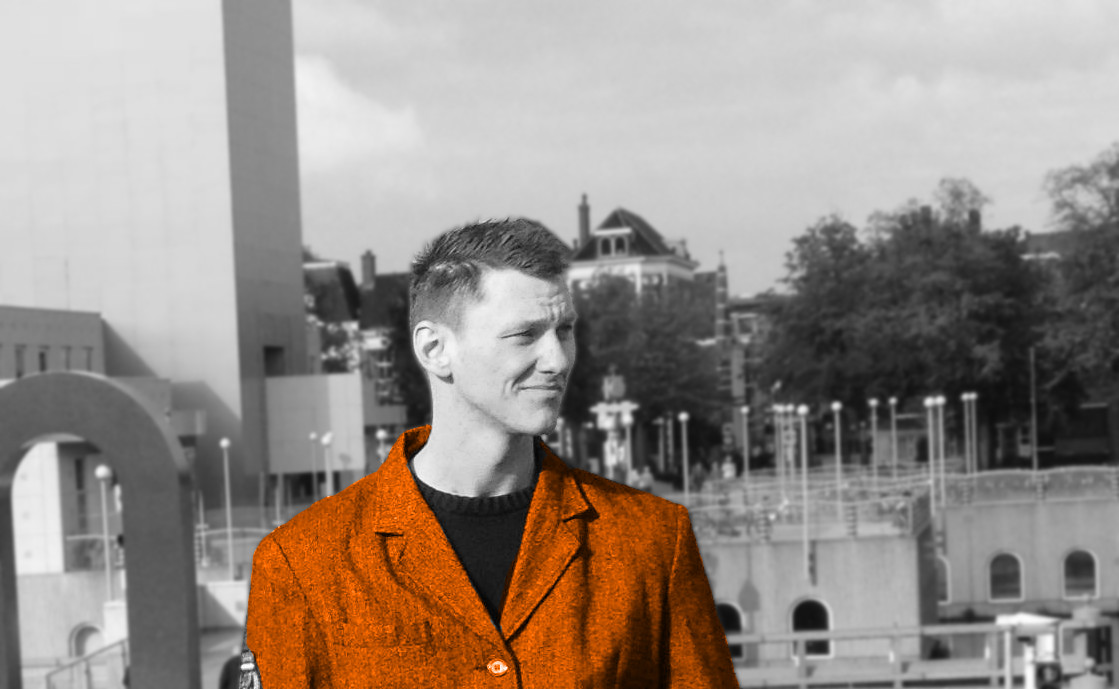
\includegraphics[trim= 0 50 0 100,clip,width=1.005\paperwidth]{myfoto.jpg}	%trimming relative to image size!
 %   \end{center}
%\end{figure}

%---------------------------------------------------------------------------------------
%	TITLE HEADLINE
%----------------------------------------------------------------------------------------
\vspace{-20.55pt}


\hspace{-0.25\linewidth}\colorbox{bgcol}{\makebox[1.5\linewidth][c]{\HUGE{\textcolor{white}{\textsc{Jan Küster}} } \textcolor{sectcol}{\rule[-1mm]{1mm}{0.9cm}} \parbox[b]{5cm}{   \large{ \textcolor{white}{{Assessment Software}}}\\
 \large{ \textcolor{white}{{Developer}}}}
}}


%---------------------------------------------------------------------------------------
%	META SECTION
%----------------------------------------------------------------------------------------
\vspace{-144pt}

\includegraphics[width=64pt]{qrcode}
\normalsize
\vspace{88pt}

\metasection{Languages:}{Flex \& AIR, Java, Processing, Latex}
\metasection{Concepts:}{Software Design, Design Pattern, Usability}
\metasection{Activities:}{FL Studio, Blender, Muay Thai, Grappling}


%---------------------------------------------------------------------------------------
%	SUMMARAY
%----------------------------------------------------------------------------------------

%\cvsection{Summary}\\
%Digital media graduate with four years project experience in the field of technology based assessment. Specialized in development of test-scenario engines and innovative, rich media item formats. Master studies focused on teams from different disciplines and cultural backgrounds on solutions for complex problems.  Prior knowledge has been collected in he field of usability / accessibility during bachelor studies.\\

%---------------------------------------------------------------------------------------
%	EXPERIENCE
%----------------------------------------------------------------------------------------

\cvsection{Experience}

\cvevent{2013 / 09}{Poster Presentation}{DELFI Conference}{Usability Guidelines for Tests with Functional Illiterates (Publication)}
{Presented results from usability field tests with functional illiterates;}


\textcolor{softcol}{\hrule}

\cvevent{2012 - Present}{Software Developer}{BMBF Project}{Technology Based Domain Specific Learning Assessment}
{Gather requirements from partners; Software design; Test engine design; Leading development team of three }
\textcolor{softcol}{\hrule}
\cvevent{2010 - 2011}{Student Assistant}{BMBF Project}{otu.lea - online test environment targeting functional illiterates}{Software design by given architecture; Implementation; Testing; Reporting}
\textcolor{softcol}{\hrule}
\cvevent{2009}{Semester Abroad}{University of Melbourne}{Studied one semester in Melbourne, Australia}{Programming the machine; Information visualization; Professional essay writing}

%---------------------------------------------------------------------------------------
%	EDUCATION 
%--------------------------------------------------------------------------------------
\cvsection{Education}

\cvevent
{2012 - Present}
{Master of Science Digital Media}
{University of Bremen}
{Thesis: Developing and Evaluating an Algorithm for Automated Scoring of Spreadsheets (in progress)}{Intercultural classes in english; Special topics in programming and design;  }
\textcolor{softcol}{\hrule}
\cvevent{2011 / 11}{Seminar on Project Management}{Getoq Consulting}{Two day simulation of a generic project lifecycle from management perspective.}{Customer contracts; change management; Communication; Controlling; Planning; Realization; Evaluation}
\textcolor{softcol}{\hrule}
\cvevent{2007 - 2011}{Bachelor of Science Digital Media}{University of Bremen}{Thesis: (Redesigning the Keyboard to Reduce the Cognitive Load and to Support the Learning Process for People with Low Usage Experience}{Programming basics; Technical basics; Design principles; Usability principles}

%-------------------------------------------------------------------------------------------------
%	ARTIFICIAL FOOTER (fancy footer cannot exceed linewidth) 
%--------------------------------------------------------------------------------------------------

\null
\vspace*{\fill}
\hspace{-0.25\linewidth}\colorbox{bgcol}{\makebox[1.5\linewidth][c]{\mystrut \small \textcolor{white}{www.jankuester.com} $\cdot$ \textcolor{white}{github.com/jankapunkt}}}

%============================================================================%
%
%	DOCUMENT END
%
%============================================================================%
\end{document}